\documentclass{article}

\usepackage{graphicx} % Required for inserting images
\usepackage{yehyun}
\usepackage{bm}

\title{Notes on Quantum Field Theory}
\author{Yehyun Choi}
\date{August 2024}

\begin{document}

\maketitle
\pagebreak


\section{Scalar Field Theory}
\subsection{Motivation, Causality}
\textcolor{red}{Lec 1, P\&S 2.1}

The field viewpoint is needed because quantum mechanics breaks causality. This can be shown from:
\begin{enumerate}
    \item Explicitly calculating the propagator between $\mathbf x$ and $\mathbf x_0$. For rational function of $x$ and $t$, $U(t)\sim e^{-m\sqrt{x^2-t^2}}$ with no cutoff\footnote{\url{https://physics.stackexchange.com/a/105049}}.
    \item Recalling that all Hermitian operators are observable; in relativity, this cannot be true because 2 spatially separated observables cannot affect each other. In other words, $\comm{O_1}{O_2}\ne 0$ for spatially separated $O_1$, $O_2$.
\end{enumerate}

With Lorentz transformations, we can prove that QFT is \textbf{causal} - in other words, if $(x-y)^2<0$, then $\comm{O(x)}{O(y)}=0$, or spacelike operators commute. To see this, we let $\phi(x)=\phi^-(x)+\phi^+(x)$, where each term corresponds to the creation and annihilation terms;
$$\phi^-(x)=\int\frac{\dd^3k}{\sqrt{(2\pi)^32\omega_k}}a_ke^{-ik\cdot x},\quad \phi^+(x)=\int\frac{\dd^3k}{\sqrt{(2\pi)^32\omega_k}}a^\dag_ke^{ik\cdot x}.$$
Then we can rewrite the commutator as 
\begin{align*}
    \comm{\phi(x)}{\phi(y)}&=\comm{\phi^-(x)+\phi^+(x)}{\phi^-(y)+\phi^+(y)}=\comm{\phi^-(x)}{\phi^+(y)}+\comm{\phi^+(x)}{\phi^-(y)}\\
    &=\phi^-(x)\phi^+(y)-\phi^-(y)\phi^+(x).
\end{align*}
However, $\phi^-(x)\phi^+(y)=\phi^-(y)\phi^+(x)$ if $(x-y)^2<0$, because there's a proper Lorentz transformation between $x-y$ and $y-x$. One could think that causality is restored as the amplitude of the particle propagating from $y$ to $x$ is exactly canceled out by the antiparticle propagating from $x$ to $y$. 

\subsection{Formulation}
\textcolor{red}{Lec 2, 3, 4, 5}

In QFT, observables are operator valued fields. We start with scalar fields - fields that are invariant under Lorentz transformations; $\phi'(x')=\phi(x)$, where $x'=\Lambda x$.

We start by requiring that the action is
\begin{enumerate}
    \item Lorentz invariant; 
    \item Causal - $S$ is local, $S=\int\dd^4 L(\phi,\partial_\mu\phi)$, with $\phi(x)$ only, no $\phi(y)$;
    \item Corresponding to EoM with 2nd order in time derivative - only possible terms are $\phi^2$ and $(\partial_\mu\phi)^2$ (note that higher order time derivatives would be one higher in length scale, $L\sim 10^{-35}$ m.)
\end{enumerate}
This is sufficient to write down the general form of the action:
$$S=\int\dd^4x\left(\frac 12\partial_\mu\phi\partial^\mu\phi-\frac{m^2}2\phi^2\right).$$
From the Euler-Lagrange equation,
$$\pde{\mathcal L}{\phi}-\partial_\mu\left(\pde{\mathcal L}{(\partial_\mu\phi)}\right)=0\implies\partial_\mu\partial^\mu\phi+m^2\phi=0.$$
This is known as the Klein-Gordon equation.

To solve the Klein-Gordon equation, we can try 
$$\phi(\mathbf x,t)=\int\frac{\dd^3k}{(2\pi)^{3/2}}e^{i\mathbf k\cdot\mathbf x}\tilde\phi(\mathbf k,t)\implies \pden 2{\tilde\phi}t+\omega_k^2\tilde\phi=0,$$
where $\omega_k^2=k^2+m^2$. Further imposing the realness conditions, we have $\tilde\phi(\mathbf k,t)=\tilde\phi^*(-\mathbf k,t)$, giving us
\begin{equation}
    \phi(\mathbf x,t)=\int\frac{\dd^3k}{\sqrt{(2\pi)^3\cdot 2\omega_k}}\left(a_ke^{-ik\cdot x}+a^*_ke^{ik\cdot x}\right),
\end{equation}
where we have defined $k^\mu=(\omega_k,\mathbf k)$ and $x^\mu=(t,\mathbf x)$. Note that the factors of $\sqrt{2\omega_k}$ and $a_k,a^*_k$ are constants chosen for convention - this is called Harmonic normalization (this normalizes $\braket{\mathbf p}{\mathbf q}$. Note that $\delta(\mathbf p)$ has units $\mathbf p^{-1}$ so it's not Lorentz invariant)

For full quantinization, we obtain $\pi(x)$, the canonical momentum field, as $\partial_{\dot\phi}\mathcal L=\pi$. For the Klein-Gordon theory,
\begin{equation}
    \pi(\mathbf x,t)=\pde{\mathcal L}{\dot\phi}=\int\frac{\dd^3k}{\sqrt{(2\pi)^3\cdot 2\omega_k}}\left(a_k(-i\omega_k)e^{-ik\cdot x}+a^\dag_k(i\omega_k)e^{ik\cdot x}\right).
\end{equation}
Imposing the canonical commutation relations\footnote{\url{https://physics.stackexchange.com/a/573940}} (\textcolor{red}{add stuff}):
\begin{equation}
    \comm{\phi(\mathbf x,t)}{\phi(\mathbf y,t)}=0,\quad\comm{\pi(\mathbf x,t)}{\pi(\mathbf y,t)}=0,\quad\comm{\phi(\mathbf x,t)}{\pi(\mathbf y,t)}=i\delta(\mathbf x-\mathbf y),
\end{equation}
we solve for the ladder operators\footnote{\url{https://physics.stackexchange.com/q/304539}}
$$a_k=i\int\frac{\dd^3x}{\sqrt{(2\pi)^3\cdot 2\omega_k}}\cdot e^{ik\cdot x}\left[\dot\phi(x)-i\omega_k\phi(x)\right],\quad a^\dag_k=-i\int\frac{\dd^3x}{\sqrt{(2\pi)^3\cdot 2\omega_k}}\cdot e^{-ik\cdot x}\left[\dot\phi(x)+i\omega_k\phi(x)\right].$$
We see that the ladder operators 
\begin{equation}
    \comm{a_k}{a^\dag_k}=\delta(\mathbf k-\mathbf k').
\end{equation}

With the conjugate momentum defined, we can write the Hamiltonian:
$$H=\int\dd^3x\left[\frac 12\pi^2+\frac 12(\nabla\phi)^2+\frac{m^2}2\phi\right]=\int\dd^3k\cdot \frac 12\omega_k(a_ka^\dag_k+a^\dag_ka_k).$$
Note that $a_ka^\dag_k=\delta(0)$ blows up. This, analogous to summing the vacuum energy density over all space and modes, is known as the cosmological constant\footnote{Turns out, the observed cosmological constant is $10^{-120}$ times smaller - this is known as the cosmological constant/fine tuning problem.} and can be canceled in the absence of gravity. This operation of canceling out the vacuum energy is called the \textbf{normal ordering} - when acted on a product of annihilation and creation operators, all the creation operators come to the front - for example, $:aa^\dag:=a^\dag a$, and so on.

The space of states in QFT is called the Fock space. The particle states $\ket k=a^\dag_k\ket 0$ are orthonormal and complete:
$$\braket{\mathbf k'}{\mathbf k}=\delta(\mathbf k-\mathbf k'),\quad \mathbbm 1=\int\frac{\dd^3k}{(2\pi)^32\omega_k}\ket{\mathbf k}\bra{\mathbf k}.$$

\textcolor{red}{Addendum about translation operator, Lec. 4}

\paragraph{Lorentz transformations}

The Lorentz transformations have a unitary representation $U(\Lambda)\ket k=\ket{\Lambda k}$ in the relativistic normalization of states - that is, there exists $U(\Lambda)$ such that $U(\Lambda_1)U(\Lambda_2)=U(\Lambda_1\Lambda_2)$ and $U^\dag U=\mathbbm 1$. We see that the following conditions are satisfied:
\begin{enumerate}
    \item Representation condition: $U(\Lambda_1)(\Lambda_2)\ket k=U(\Lambda_1\Lambda_2)\ket k$, follows from the definition;
    \item Unitarity: First, note that relativistic integrand is Lorentz invariant, as $\frac{\dd^3k}{(2\pi)^32\omega_k}=\dd^4k\delta(k^2-m^2)$. Then, from the completeness relation, 
    $$UU^\dag=\int\frac{\dd^3}{(2\pi)^32\omega_k}\ket{\Lambda k}\bra{\Lambda k}=\int\frac{\dd^3k'}{(2\pi)^32\omega_k}\ket{k'}\bra{k'}=\mathbbm 1,$$
    where $k'=\Lambda k$. 
\end{enumerate}
Note that relativistic creation/annihilation operators and field operators follow
$$\alpha^\dag(\Lambda k)=U(\Lambda)\alpha^\dag_kU(\Lambda)^{-1},\quad U\phi U^\dag=\phi(\Lambda x).$$
In other words, $\phi(x)$ transforms like a scalar.

\subsection{Symmetries and Conservation Laws}
\subsubsection{Continuous Symmetries}
\textcolor{red}{Lec 6, }

As far as symmetries and conservation laws are concerned, we note that
\begin{enumerate}
    \item Symmetries have unitary representations\footnote{Stated by Wigner's theorem. }; for $U(R)$ corresponding to rotation $R$, $U(R_1)U(R_2)=U(R_1R_2)$ and $U^\dag U=\mathbbm 1$.
    \item Symmetries should leave the dynamics unchanged; for $\ket\psi=U\ket\phi,$ $e^{-iHt}\ket{\psi}=Ue^{-iHt}\ket\phi\implies U^\dag HU=H$.
\end{enumerate}
For a continuous symmetry, we can also write $R\sim\mathbbm 1+i\epsilon T$, where $T$ is the infinitesimal generator of symmetry. We can also relate infinitesimal symmetry to a discrete one by exponentiating - $R=e^{i\epsilon T}$. The generators are a Lie algebra, closed under the Lie bracket; $\comm{T^a}{T^b}=if^{abc}T^c$, where $f^{abc}$ is the structure constant; in SO(3), this is the Levi-Civita symbol. The generators for a unitary transformation are called charge operator:
$$U(\mathbbm 1+i\epsilon T)=1+i\epsilon Q,\quad U^{-1}=U^\dag\implies Q=Q^\dag.$$
Further imposing the dynamics condition, we have $\comm{Q}{H}=0$. 

Furthermore, the finite transformations $R=e^{i\epsilon T}$ form a Lie group - they are related to Lie algebra by the BCH formula. Lie groups are also closed under (matrix) multiplication; $R(h)R(g)=R(h\circ g)\implies e^{i\epsilon T^a}e^{i\epsilon T^b}=e^{i\epsilon T^c}$. 

\subsubsection{Conservation Laws}
Recall that if the Lagrangian changes by a total derivative, the action doesn't change. Explicitly, we have 
$$\delta\mathcal L=\pde{\mathcal L}{\phi_a}\delta\phi^a+\pde{\mathcal L}{(\partial_\mu\phi^a)}\partial_\mu\delta\phi^a=\partial_\mu F^\mu\implies\partial_\mu\left(\pde{\mathcal L}{(\partial_\mu\phi^a)}\delta\phi^a-F^\mu\right)\equiv \partial_\mu J^\mu=0.$$
We define $J^\mu$ to be the \textbf{Noether current}. The corresponding conserved charge can be found $Q=\int\dd^3xJ^0$.

As an example, we look at \textbf{translational symmetries}. If the action has no explicit $x$ dependency, we can vary the fields 
$$\phi^a(x^\mu+\epsilon a^\mu)\sim \phi^a(x^\mu)+\epsilon a^\mu\partial_\mu\phi^a,\quad \mathcal L(x^\mu+\epsilon a^\mu)\sim\mathcal L(x)+\epsilon a^\mu\partial_\mu\mathcal L.$$
Hence, $\delta\phi^a=a^\mu\partial_\mu\phi^a$, and $F^\mu=a^\mu\mathcal L$. The corresponding Noether current can be found to be 
$$J^\nu=\pde{\mathcal L}{(\partial_\nu\phi^a)}\delta\phi^a-F^\nu=\pde{\mathcal L}{(\partial_\nu\phi^a)}a^\mu\partial_\mu\phi^a-a^\nu\mathcal L=a^\mu T_\mu^\nu,\quad T^\mu_\nu=\pde{\mathcal L}{(\partial_\nu\phi)}\partial_\mu\phi-\delta^\nu_\mu\mathcal L.$$
We define $T^\mu_\nu$ to be the \textbf{stress-energy tensor}. From $\partial_\nu J^\nu=0$, it holds that $\partial_\nu T^\mu_\nu=0$ as well. The conserved charge, or the 4-momentum in this case, can be found 
$$\int\dd^3x T^{\mu 0}=p^\mu,\quad\partial_tp^\mu=0.$$
As an example, for a real scalar field, 
$$:H:=\int\dd^3k\cdot \omega_ka^\dag_k a_k,\quad :p^\mu:=\int\dd^3k\cdot k^\mu a^\dag_ka_k.$$

\subsubsection{Discrete Symmetries}
\textcolor{red}{2nd half Lec 7}

There also exists discrete symmetries associated with Lorentz transformations, defined $\Lambda^\intercal g\Lambda=g$. The first is the \textbf{parity reversal}, defined, for a scalar field, as a unitary, linear operator that satisfies
$$U_p:\phi(t,\mathbf x)\mapsto\phi(t,-\mathbf x)\implies U_p:a_k,a^\dag_k\mapsto a_{-k},a^\dag_{-k}$$
where we let $\mathbf k\to-\mathbf k$ in the field integral.

Next, we have the \textbf{time reversal}, defined as a unitary, anti-linear operator that satisfies
$$U_t:\phi(t,\mathbf x)\mapsto\phi^*(-t,\mathbf x)\implies U_t:a_k,a^\dag_k\mapsto a_{-k},a^\dag_{-k},$$
where $k\sim\dot x\to-k$ and $i\to-i$ in this transformation. 

Lastly, the \textbf{charge conjugation} is a unitary operator, defined for complex fields, that satisfies
$$U_c:\psi(t,\mathbf x)\mapsto\psi^\dag(t,\mathbf x),\quad U_c:b_k,b^\dag_k\mapsto c_k,c^\dag_k.$$

For non-interacting theories, all combinations of C, P, and T are symmetries. However, for interacting theories, C, P, and CP can be broken, but never \textbf{CPT}.

\subsection{Complex Scalar Fields}
\textcolor{red}{1st half Lec 7, }

While we have found symmetries with $x$-dependence so far, another group of symmetries, called \textbf{internal symmetries} exist. As a motivation, consider a system consisting of two real (independent), identical scalar fields:
$$\mathcal L=\frac 12(\partial_\mu\phi^1)^2+\frac 12(\partial_\mu\phi^2)^2-\frac 12m_1^2\phi_1^2-\frac 12m_2^2\phi_2^2.$$
It is possible to ``rotate'' - $U(1)\sim SO(2)$ symmetry two fields into each other: $\begin{pmatrix}\phi^1\\\phi^2\end{pmatrix}\to\begin{pmatrix}\cos\theta&\sin\theta\\-\sin\theta&\cos\theta\end{pmatrix}\begin{pmatrix}\phi^1\\\phi^2\end{pmatrix}.$ The current and charge associated with this symmetry is 
$$J^\mu=(\partial^\mu\phi^1)\phi^2-(\partial^\mu\phi^2)\phi^1,\quad Q=-i\int\dd^3k(a^{2\dag}_ka^1_k-a^{1\dag}_ka^2_k).$$
Because $\comm{H}{Q}=0$, it is possible to diagonalize the charge operator; let 
$$b_k=\frac 1{\sqrt 2}(a^1_k+ia_k^2),\quad c_k=\frac 1{\sqrt 2}(a^1_k-ia^2_k).$$
whThe commutation relations still hold:
$$\comm{b}{b}=\comm{c}{c}=\comm{b}{c^\dag}=0,$$
and each operator corresponds to creating/annihilating a $+1$ charge ($b,b^\dag$) or a $-1$ charge ($c,c^\dag$) particle.

With these new definitions, we can write 
$$Q=\int\dd^3k(b^\dag_kb_k-c^\dag_kc_k),\quad:H:=\int\dd^3k\cdot\omega_k(b^\dag_kb_k+c^\dag_kc_k).$$
Furthermore, we can define the field operator as 
$$\psi=\frac 1{\sqrt 2}(\phi^1+i\phi^2),\quad\psi=\int\frac{\dd^3k}{\sqrt{(2\pi)^32\omega_k}}(b_ke^{ik\cdot x}+c^\dag_ke^{-ik\cdot x}),\quad \psi^\dag=\int\frac{\dd^3k}{\sqrt{(2\pi)^32\omega_k}}(b^\dag_ke^{-ik\cdot x}+c_ke^{ik\cdot x}),$$
with commutation relations
$$\comm{\psi}{\psi}=\comm{\psi^\dag}{\psi^\dag}=0,\quad\comm{\psi(x,t)}{\dot\psi^\dag(y,t)}=i\delta(x-y).$$
The $\psi$ field creates an anti-particle ($c^\dag$) and annihilates particle ($b$), and the opposite for $\tilde\psi$. 

As a side note, when written as a complex scalar, the ``rotation internal symmetry'' becomes a simple phase factor - they are $SO(2)\sim U(1)$ symmetries - $R\psi = \psi e^{-i\theta}$, where $R$ is the motivating rotation matrix. 

We can write the Lagrangian density and the rotation symmetry:
$$\mathcal L=\partial_\mu\psi^\dag\partial^\mu\psi-m^2\psi^\dag\psi,\quad J_\mu= i\left[\psi\partial_\mu\psi^\dag-\psi^\dag\partial_\mu\psi\right].$$

\pagebreak

\section{Interacting Fields}
\subsection{Formulation}
\textcolor{red}{Lec 8,9}

For a system with an interaction, term, the Hamiltonian can be written $H=H_0+H_\text{int}$. We define the interaction action field to be 
$$\phi_I(t,\mathbf x)=e^{iH_0(t-t_0)}\phi(t_0,\mathbf x)e^{-iH_0(t-t_0)}=e^{iH_0(t-t_0)}\left(e^{-iH(t-t_0)}\phi(t,\mathbf x)e^{iH(t-t_0)}\right)e^{-iH_0(t-t_0)}.$$
In other words, the interaction field is what the field would evolve (from $t_0$ to $t$) if it weren't for the interacting terms. Now, we define the time evolution operator, which gives a concise expression of the full field:
$$U(t,t_0)=e^{iH_0(t-t_0)}e^{-iH(t-t_0)}\implies \phi(t,\mathbf x)=U^\intercal(t,t_0)\phi_I(t,\mathbf x)U(t,t_0).$$
Taking the derivative of the time evolution operator, 
$$i\pde{}tU(t,t_0)=\left(e^{iH_0(t-t_0)}H_\text{int} e^{-iH_0(t-t_0)}\right)U(t,t_0)=H_I(t)U(t,t_0),$$
we can see that $H_I(t)$ is the interaction Hamiltonian written in the interaction picture - evolving with the free Hamiltonian. The solution for this differential equation - with $U(t_0,t_0)=1$ - is a power series:
\begin{align*}
    U(t,t_0)=&1+(-i)\int^t_{t_0}\dd t_1\,H_I(t_1)+(-i)^2\int^t_{t_0}\dd t_1\int^{t_1}_{t_0}\,\dd t_2H_I(t_1)H_I(t_2)\\
    &+(-i)^3\int^t_{t_0}\dd t_1\int^{t_1}_{t_0}\dd t_2\int^{t_2}_{t_0}\dd t_3\,H_I(t_1)H_I(t_2)H_I(t_3)+\cdots.
\end{align*}
Note that the successive integration limits get smaller and the interaction Hamiltonians are time-ordered. To get rid of the time-ordering operators, we note that 
$$\int^t_{t_0}\dd t_1\int^{t_1}_{t_0}\dd t_2\cdots\int^{t_{n-1}}_{t_0}\dd t_n\,H_I(t_1)\cdots H_I(t_n)=\frac 1{n!}\int^t_{t_0}\dd t_1\cdots\dd t_n T\left[H_I(t_1)\cdots H_I(t_n)\right].$$
Refer to Peskin 4.21 for a ``proof''\footnote{\url{http://scipp.ucsc.edu/~haber/ph215/TimeOrderedExp.pdf}} - it is analogous to finding the volume of an $n$-simplex. With this, we can write $U(t,t_0)$ in a compact form:
\begin{align*}
    U(t,t_0)&=1+(-i)\int^t_{t_0}\dd t_1\,H_I(t_1)+\frac{(-i)^2}{2!}\int^t_{t_0}\dd t_1\dd t_2\,T[H_I(t_1)H_I(t_2)]+\cdots\\
    &=T\exp\left(-i\int^t_{t_0}\dd t'H_I(t')\right)=T\exp\left[i\int^t_{t_0}\int\dd^3x'\mathcal L'(\phi_I(\lambda'))\right]
\end{align*}
Note that 
\begin{itemize}
    \item In this form, it is evident (from the limits of integrals) that $U(t_1,t_2)U(t_2,t_3)=U(t_1,t_3),$ and $U(t_1,t_3)U^\dag(t_2,t_3)=U(t_1,t_2);$
    \item The time ordering operator is invariant - order of events doesn't change for timelike events and all $\phi$ commute for spacelike events - the Lagrangian is invariant, and the integral $\int\dd t\int\dd x'$ is invariant if we let $t,t_0$ to $\pm\infty$.
\end{itemize}

We first claim that as $t\to\pm\infty$, interactions effectively turn off; asymptotically, we will have free field/particles, each state approaching the asymptotic state\footnote{This really isn't true because of self and vacuum interactions, but we will come back here for renormalization.}. If we let $\ket\psi$ as the free states and $\ket\psi_\text{in}$ and $\ket\psi_\text{out}$ as the interacting states, we have 
$$\lim_{t\to-\infty}e^{-iHt}\ket{\psi(t=0)}_\text{in}=e^{-iH_0t}\ket{\psi(t=0)},\quad \lim_{t\to\infty}e^{-iHt}\ket{\psi(t=0)}_\text{out}=e^{-iH_0t}\ket{\psi(t=0)}.$$
In other words, 
$$\ket\psi_\text{in}=\lim_{t\to-\infty}e^{iHt}e^{-iH_0t}\ket\psi,\quad\ket\psi_\text{out}=\lim_{t\to\infty}e^{iHt}e^{-iH_0t}\ket\psi.$$
We're interested in scattering amplitudes, defined as the probability of measuring $\ket\chi_\text{out}$ given an in state $\ket\psi_\text{in}$. We have 
$$\braket{\chi_\text{out}}{\psi_\text{in}}=\lim_{t'\to-\infty}\lim_{t\to\infty}\bra\chi U(t,t')\ket\psi=S_{\chi\psi},$$
where we define $S=\lim_{t,t\to\pm\infty}U(t,t')$, which is also called the $S$ or scattering matrix. The $S$-matrix is unitary; $S^\dag S=\mathbbm 1$, and commutes with/preserves free energy; $\comm{S}{H_0}=0$. Therefore, 
\begin{equation}
    S=T\exp\left[i\int^\infty_{-\infty}\dd^4x\mathcal L(\Phi_I)\right].
\end{equation}
This is known as Dyson's equation. 

Recall that $\Phi_I$ are fields that can be expressed in ladder operators, which are easier to work with in normal ordering. For this, we introduce \textbf{Wick's theorem}, a theorem that relates time ordering $T$ to normal ordering $::$. First, we define the \textbf{contraction}, defined 
$$T(\phi^a(x)\phi^b(y))=:\phi^a(x)\phi^b(y):+\wick{\c1\phi^a(x)\c1\phi^b(y)}.$$
We can find an explicit form for the contraction:
\begin{itemize}
    \item For the $x^0>y^0$ case, we have 
    \begin{align*}
        T[\phi^a(x)\phi^b(y)]&=\phi^a(x)\phi^b(y)=\left(\phi^{a+}(x)+\phi^{a-}(x)\right)\left(\phi^{b+}(x)+\phi^{b-}(y)\right)=:\phi^a\phi^b:+\delta_{ab}\Delta_+(x-y),
    \end{align*}
    \item For $x^0<y^0$, we have 
    $$T[\phi^a(x)\phi^b(y)]=\normord{\phi^a\phi^b}+\delta_{ab}\Delta_+(y-x).$$
\end{itemize}
Hence, we obtain
$$\wick{\c1\phi^a(x)\c1\phi^b(y)}=\delta_{ab}\int\frac{\dd^4k}{(2\pi)^4}e^{-ik(x-y)}\frac{i}{k^2-m^2+i\epsilon}.$$
Now, we can state Wick's theorem:
\begin{align}
\begin{split}
    T(\phi_1\cdots\phi_n)=&:\phi_1\cdots\phi_n:\\
    &+\wick{\c1\phi_1\c1\phi_2}:\phi_3\cdots\phi_n:+\wick{\c1\phi_1\c1\phi_3}:\phi_2\phi_4\cdots\phi_n:+\cdots\\
    &+\wick{\c1\phi_1\c1\phi_2}\wick{\c1\phi_3\c1\phi_4}:\phi_5\cdots\phi_n:\\
    &\vdots
\end{split}
\end{align}
We prove this by induction. Consider $n$ fields $\phi_1,\cdots,\phi_n$ with times $\phi_1^0\ge \phi_2^0\ge,\cdots\phi_n^0$. If $\phi_2\cdots\phi_n$ were in Wick-expression - $T\phi_1\phi_2=:\phi_1\phi_2:+\wick{\c1\phi_1\c1\phi_2)}$, which is the zeroth term, is in Wick ordering by definition - we can multiply by $\phi_1$ on the left. Since all fields are time-ordered already,
$$T(\phi_1\cdots\phi_n)=\phi_1(:\phi_2\cdots\phi_n:+\wick{\c1\phi_2\c1\phi_3:\phi_4\cdots\phi_n:+\cdots}).$$
Now, let $\phi_1^+$ and $\phi_1^-$ be the creation/annihilation parts of $\phi_1$. Then, we have 
\begin{align*}
    T(\phi_1\cdots\phi_n)=\phi_1^+:\phi_2\cdots\phi_n:+\phi_1^-:\phi_2\cdots\phi_n:+\phi_1+(\phi^+_1+\phi^-_1)\wick{\c1\phi_2\c1\phi_3:\phi_4\cdots\phi_n:+\cdots}.
\end{align*}
Let's focus on the non-contraction terms for a minute. They can be written 
$$\phi^+_1\normord{\phi_2\cdots\phi_n}+\phi^-_1\normord{\phi_2\cdots\phi_n}=\normord{\phi^+_1\phi_2\cdots\phi_n}+\normord{\phi_2\cdots\phi_n\phi^-_1}+\comm{\phi^-_1}{\normord{\phi_2\cdots\phi_n}}.$$
From definition, the first two terms are $\normord{\phi_1\phi_2\cdots\phi_n}$. The commutator can be explicitly evaluated:
\begin{align*}
    \comm{\phi^-_1}{\normord{\phi_2\cdots\phi_n}}&=\comm{\phi^-_1}{\phi^+_2\normord{\phi_3\cdots\phi_n}}+\comm{\phi^-_1}{\phi^-_2\normord{\phi_3\cdots\phi_n}}\\
    &=\comm{\phi^-_1}{\phi^+_2}\normord{\phi_3\cdots\phi_n}+(\phi^+_2+\phi^-_2)\comm{\phi^-_1}{\normord{\phi_3\cdots\phi_n}}+\Ccancel[red]{\comm{\phi^-_1}{\phi^-_2}\normord{\phi_3\cdots\phi_n}}.
\end{align*}
Using the fact that $\comm{\phi^-_1}{\phi^+_2}=\wick{\c1\phi_1\c1\phi_2}$ for $x^0_1>x^0_2$, we get 
$$\comm{\phi^-_1}{\normord{\phi_2\cdots\phi_n}}=\sum^n_{i=2}\phi_2\cdots\phi_{i-1}\wick{\c1\phi_1\c1\phi_i}\phi_{i+1}\cdots\phi_n.$$
Keeping in mind that all contractions are complex numbers, we can deduce that the contraction terms are 
$$(\phi^+_1+\phi^-_1)\wick{\c1\phi_2\c1\phi_3}\normord{\phi_4\cdots\phi_n}+\cdots=\wick{\c1\phi_2\c1\phi_3}\normord{\phi_1\phi_4\cdots\phi_n}+\wick{\c1\phi_2\c1\phi_3}\sum^n_{i=4}\phi_4\cdots\phi_{i-1}\wick{\c1\phi_1\c1\phi_i}\phi_{i+1}\cdots\phi_n+\cdots.$$
In other words, multiplying a normal ordered sequence by $\phi_1$ is the normal ordering sequence with $\phi_1$ and all single contractions with $\phi_1$. Hence Wick's theorem is proved.

\subsubsection{Interaction with External Field}
\textcolor{red}{Lec 9, 10}

Let the interacting Hamiltonian of the external field be $H'=\lambda\phi(x)\rho(x)$. For boundary conditions, we let $\rho(x)\to 0$ for $t\pm\infty$. From Dyson's formula, we have 
$$S=T\sum^\infty_{n=0}\frac{(-i\lambda)^n}{n!}\left(\int\rho(x)\phi(x)\cdot\dd^3x\right)^n.$$ 
From Wick's formula, we have to sum over every possible number of contractions:
$$\sum_{n,p}\frac{(-i\lambda)^n}{n!}\left(\int\dd^4x_1\,\dd^4x_2\,\rho(x_1)\rho(x_2)\wick{\c1\phi(x_1)\c1\phi(x_2)}\right)^p\normord{\left(\int\dd^4x_3\rho(x_3)\phi(x_3)\right)^{n-2p}}\frac{n!}{2^p(n-2p)!p!}.$$
Note that the combinatoric factor can be considered by choosing $p$ pairs from $n$ objects:
$$\binom n2\binom{n-2}2\cdots\binom{n-(2p-2)}2\cdot\frac 1{p!}=\frac{n!}{2^p(n-2p)!p!}.$$
If we redefine $k=n-2p$, we get 
$$S=A\normord{\exp\left(-i\lambda\int\dd^4x\,\rho(x)\phi(x)\right)},\quad A=\exp\left(\frac 12(-i\lambda)^2\int\dd^4x_1\,\dd^4x_2\,\rho(x_1)\rho(x_2)\wick{\c1\phi(x_1)\c1\phi(x_2)}\right).$$
The Fourier transformation of the $\rho(x)$ is $\rho(x)=\int\frac{\dd^4k}{(2\pi)^4}\tilde\rho(k)e^{-ikx}$, we have 
$$\int\dd^4x\,\rho(x)\phi(x)=\int\frac{\dd^3k}{(2\pi)^32\omega_k}(\tilde\rho(-k)a_k+\tilde\rho(k)a^\dag_k)$$
From this, we can calculate the probability of creating $n$ particles: $\bra{k_1\cdots k_n}S\ket 0$; since the $S$ matrix is acting on the vacuum state, we want to have $n$ creation operators that exactly match the momenta $k_1\cdots k_n$; 
$$\bra{k_1\cdots k_n}S\ket 0=A\tilde\rho(k_1)\cdots\rho(k_n)(-i\lambda)^n\implies\bra{k_1}S\ket 0=-i\lambda A\tilde\rho(k_1).$$

Recall that $\bra{k_1k_2}S\ket 0\sim\tilde\rho(k_1)$, which is the Fourier transform of the source. For a static source, no particles are created, but the ground/vacuum energy changes:
$$\bra 0S\ket 0=A=\exp\left(\frac{(-i\lambda)^2}{2}\int\frac{\dd^4k}{(2\pi)^4}\abs{\tilde f(k^0)}^2\abs{\tilde\rho(k)}^2\frac{i}{k^2-m^2+i\epsilon}\right)=\exp\left(-i(\gamma_\text{on}+\gamma_\text{off}+E_0T)\right).$$
This can be interpreted as the phase from turning the source on/off plus the phase from $E_0T$, where $T$ is the duration of the source. We have 
$$E_0=\frac{(-i\lambda)^2}{2T}\int\frac{\dd^4k}{(2\pi)^4}\abs{f(k^0)}^2\abs{\tilde\rho(\mathbf k)}^2\frac{i}{k^2-m^2+i\epsilon}+\Ccancel[red]{\frac{-\gamma_\text{on}-\gamma_\text{off}}{T}}.$$
From Parseval's theorem\footnote{\url{https://mathworld.wolfram.com/ParsevalsTheorem.html}}, we have 
$$E_0=-\frac{\lambda^2}{2}\int\frac{\dd^3k}{(2\pi)^0}\abs{\rho(\mathbf k)}^2\frac 1{k^2+m^2-i\epsilon}=\frac{\lambda^2}2\int\rho(x_1)\rho(x_2)V(\mathbf x_1-\mathbf x_2)\dd^3x_1\dd^3x_2.$$
From the Fourier transform, we have 
$$V(\mathbf x)=-\int\frac{\dd^3k}{(2\pi)^3}e^{i\mathbf k\cdot\mathbf x}\frac 1{\mathbf k^2+m^2-i\epsilon}=-\int^\infty_{-\infty}=\frac 1{(2\pi)^2}\frac 1{ir}\frac{k\dd k}{k^2+m^2}e^{ikr}=-\frac 1{4\pi r}e^{-mr}.$$

\subsection{Feynman Diagrams}
\textcolor{red}{Lec. 11-12}

We are often interested in the (nontrivial) elements of the S-matrix as it relates to the scattering amplitude of a specific process:
$$\bra fS-\mathbbm 1\ket i=i(2\pi)^4\delta(k_f-k_i)A_{fi},$$
where $A_{fi}$ is the scattering amplitude; the momentum-conserving delta function follows from the translational invariance of the S-matrix.

Often, we represent scattering process with a Feynman diagram. To find the corresponding element of the S-matrix $\bra fS-\mathbbm 1\ket i$, 
\begin{enumerate}
    \item Draw all topologically distinct diagrams;
    \item For each vertex, add $(-i\lambda)\int\dd^4x$;
    \item For each internal line, add $\wick{\c1\phi(x_i)\c1\phi(x_j)}=\int\frac{\dd^4k}{(2\pi)^4}\frac{e^{-ik(x_i-x_j)}}{k^2-m^2+i\epsilon}$;
    \item For each incoming external line, add $e^{-ik_\alpha x_i}$; for each outgoing external line, add $e^{ik_\alpha x_i}$;
    \item Divide by the symmetry factor.
\end{enumerate}
In momentum space, the Feynman rules are much simpler; to find the scattering amplitude \textcolor{red}{times $i$} $iA_{fi}$, 
\begin{enumerate}
    \item Draw all topologically distinct diagrams;
    \item For each vertex, add $(-i\lambda)$;
    \item For each internal line, add $\frac{i}{k^2-m^2+i\epsilon}$;
    \item For each undetermined/loop momentum, integrate - $\int\frac{\dd^4k}{(2\pi)^4}$;
    \item Divide by the symmetry factor.
\end{enumerate}

\begin{figure}[h]
    \centering
    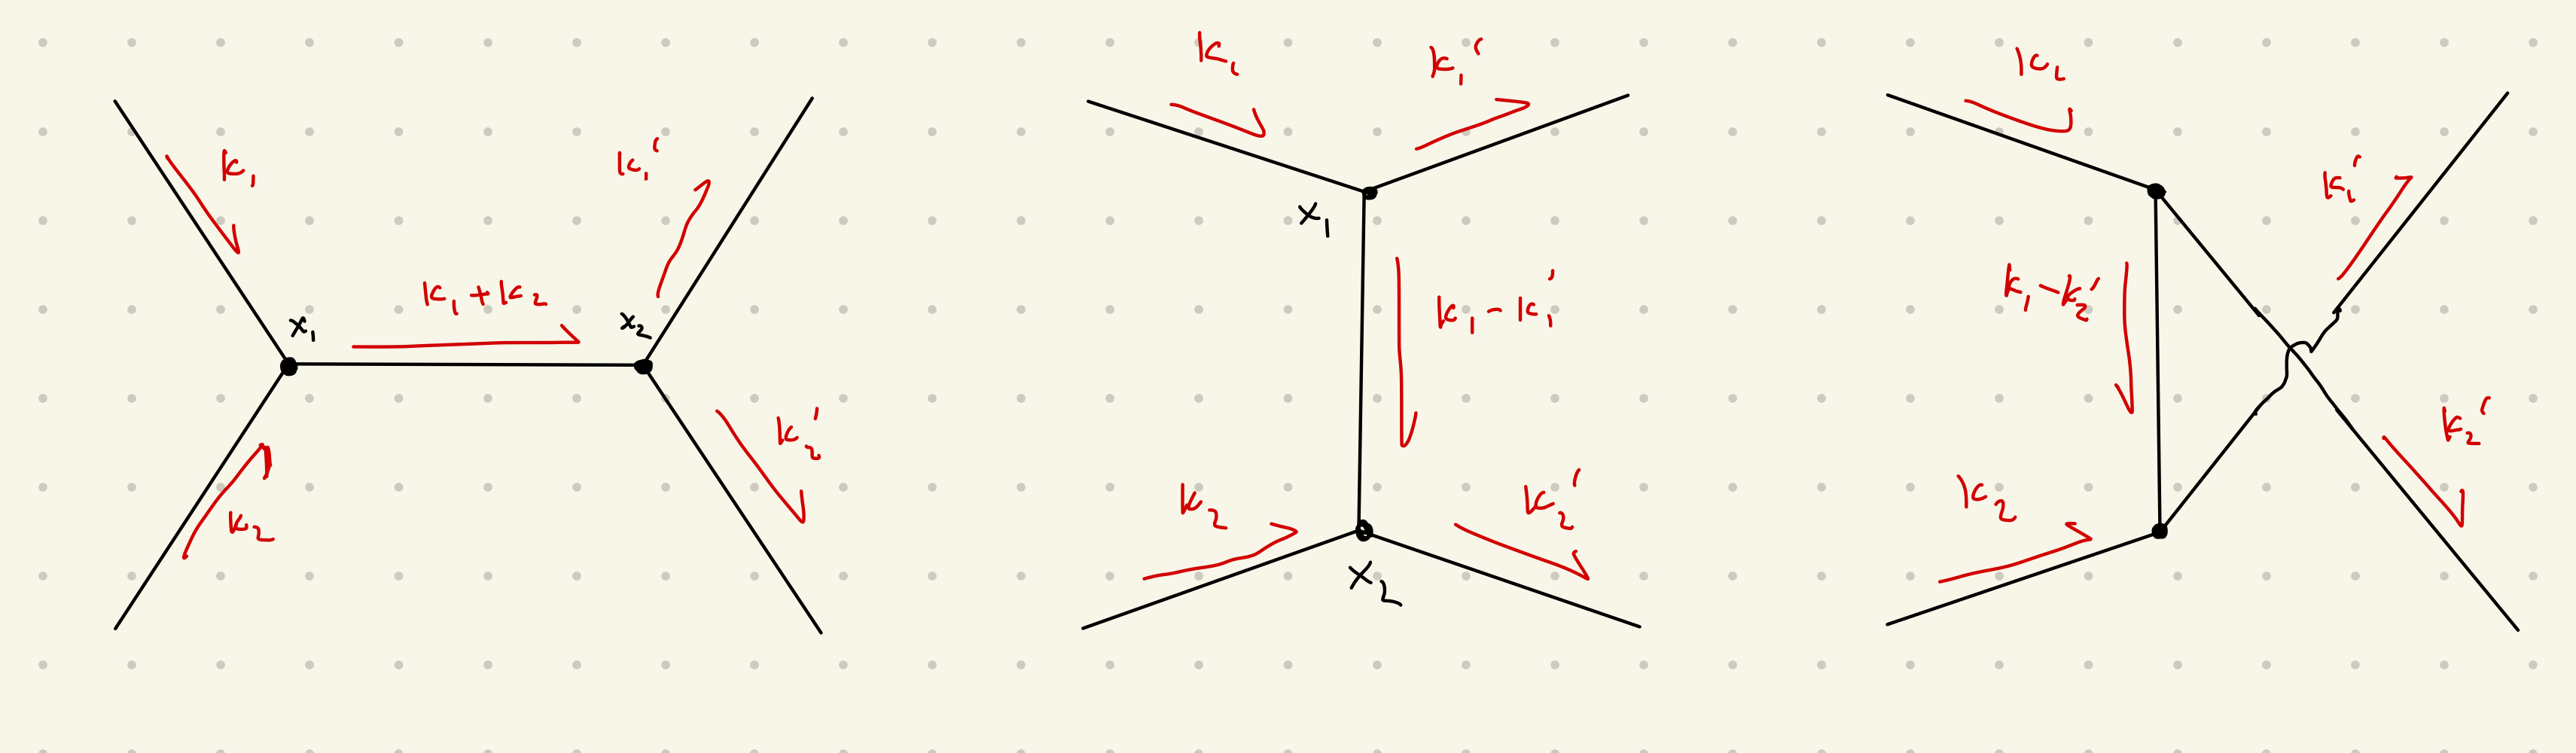
\includegraphics[width=0.95\linewidth]{images/qft-images/stuchannels.jpg}
    \caption{Feynman diagrams for the $\lambda^2$ order 2-2 scattering in $\lambda^3\phi^3/3!$ theory, also known as the S, T, and U channel}
    \label{fig:stuchannels}
\end{figure}

\example Consider the $\lambda^2$ order 2-2 scattering in $\phi^3$ theory with identical particles, as shown in figure \ref{fig:stuchannels}. The total scattering amplitude is 
$$A_{fi}=(-i\lambda)^2\cdot i\left(\frac{1}{(k_1+k_2)^2-m^2+i\epsilon}+\frac{1}{(k_1-k'_1)^2-m^2+i\epsilon}+\frac 1{(k_1-k'_2)^2-m^2+i\epsilon}\right).$$
The scattering amplitude for these processes are often written in terms of the \textbf{Mandelstam variables}. To get an intuition, we consider an elastic collision in the center of mass frame. The momenta can be written 
$$k_1=(E,0,0,p),\quad k'_1=(E,p\sin\theta,0,p\cos\theta),\quad k_2=(E,0,0,-p),\quad k'_2=(E,-p\sin\theta,0,-p\cos\theta),$$
where $\theta$ is the scattering angle. We now write the definition of the Mandelstam variables and write them in terms of $E$, $p$, and $\theta$:
\begin{align*}
    s&=(k_1+k_2)^2=4E^2=E_T^2;\\
    t&=(k_1-k'_1)^2=-4p^2\sin^2\left(\frac\theta 2\right)=-\mathbf q'^2\\
    u&=(k_1-k'_2)^2=-4p^2\cos^2\left(\frac\theta 2\right)=-\mathbf q_c^2,
\end{align*}
where $E_T$ is the total energy, $\mathbf q$ is the momentum transfer from $p_1$ to $p'_1$ and $\mathbf q_c$ is the momentum transfer in the cross channel. In terms of these variables, the scattering amplitude is 
$$A_{fi}=-i\lambda^2\left(\frac 1{s-m^2}+\frac 1{t-m^2}+\frac 1{u-m^2}\right)=-i\lambda^2\left(\frac 1{E_T^2-m^2}+\frac 1{\mathbf q^2-m^2}+\frac 1{\mathbf q_c^2-m^2}\right).$$
Note that
\begin{itemize}
    \item The s-channel amplitude, while having no direct approximation in Born approximation, simplifies to the perturbation term.
    \item The t-channel scattering amplitude can be written 
    $$\frac 1{\mathbf q^2+m^2}=\int\dd^3xe^{i\mathbf q\cdot\mathbf x}\left(\frac{e^{-mr}}{4\pi r}\right);$$
    in other words, the t-channel amplitude is the Fourier transform (Born-Oppenheimer approximation) of the Yukawa potential;
    \item The u-channel amplitude is necessary for Bose symmetry;
    \item s,t,u are not independent; $s+t+u=4m^2=m^2_1+m_2^2+m_3^2+m_4^2$, in general;
    \item The scattering amplitude is invariant under $s\leftrightarrow t\leftrightarrow u$. This is called a \textbf{crossing symmetry}. 
\end{itemize}

\subsection{Physical Quantities}
\textcolor{red}{Lec. 13-14}

Because the transition amplitude is not $L^2$, it is necessary to work in box normalization, characterized by
\begin{itemize}
    \item Periodic boundary conditions: $\mathbf k=\frac{2\pi}L\mathbf n$;
    \item Box commutation relations: $\comm{a^\text{box}_k}{a^{\dag\text{box}}_{k'}}=\delta_{kk'}$;
    \item State density $\dd n=\frac V{(2\pi)^3}\dd^3k$.
\end{itemize}
Furthermore, the Feynman rules don't change in box normalization; only the external states are changed:
$$\bra 0\phi(x)\ket k=e^{-ik\cdot x}\to \frac 1{\sqrt{2\omega_kV}}e^{-ik\cdot x}.$$
Therefore, 
\begin{align*}
    \bra fS-\mathbbm 1\ket i&=i(2\pi)^4A_{fi}\delta^{(4)}(k_\text{in}-k_\text{out})\prod_i\frac 1{\sqrt{2E_iV}}\\
    \implies \abs{\bra fS-\mathbbm 1\ket i}^2&=\abs{A_{fi}}^2(2\pi)^4\delta(k_\text{in}-k_\text{out})\cdot VT\cdot\prod_i\frac 1{(2E_iV)}
\end{align*}
where the index $i$ is over all external states and we have used $\delta^2k=\delta(k)\delta(0)=\frac 1{(2\pi)^4}\int \dd^4x=\frac{VT}{(2\pi)^4}$. Furthermore, for a measurable quantity, we should cancel out $V$ and $T$; the quantity we are interested in, the \textbf{differential transitional probability}, is obtained from the transitional probability by
\begin{itemize}
    \item Dividing by $T$; 
    \item Dividing by the flux of the initial particles;
    \item Multiplying by the density of the state factor for final states, $\dd N=\frac V{(2\pi)^3}\dd^3k$,
\end{itemize}
which ensures that the quantities are intrinsic to the process.

\begin{equation}
    V\prod_\text{init.}\frac 1{(2E_iV)}\abs{A_{fi}}^2\cdot D^{(n)},\quad D^{(n)}=\prod_i\left(\frac{\dd^3k_i}{(2\pi)^32E_i}\right)\cdot(2\pi)^4\delta^{(4)}(k_\text{in}-k_\text{out}),
\end{equation}
where $D^{(n)}$ is the \textbf{n-body phase space}, which is equal to the probability of scattering into a phase volume. We have that 
\begin{enumerate}
    \item The rate of a particle decaying into $n$ is 
    $$\dd\Gamma=\frac 1{2E_i}\abs{A_{fi}}^2D^{(n)};$$
    from $\dd\Gamma$, we obtain $\Gamma$, the decay width, from which we get $\tau=\frac 1\Gamma$, the characteristic lifetime of a particle. 
    \item The scattering cross section of a two-particle initial state is 
    $$\dd\sigma=\frac 1{4E_Tk_i}\abs{A_{fi}}^2D^{(n)},$$
    in the center of mass frame.
\end{enumerate}


\example Two-body phase space can be calculated (in the center of momentum frame),
$$D^{(2)}=\frac{\dd^3k_1}{(2\pi)^32E_1}\frac{\dd^3k_2}{(2\pi)^32E_2}(2\pi)^4\delta^{(3)}(k_1+k_2)\delta(E_1+E_2-E_T)=\frac{k^2\dd k\dd\Omega}{(2\pi)^2\cdot 2E_1\cdot 2E_2}\delta(E_1+E_2-E_T).$$
Further writing $\delta(E)$, we have $\delta(E_1+E_2-E_T)=\frac{\delta(k-k_0)}{\abs{\partial_kE_1+\partial_kE_2}_{k=k_0}}$. With $\ode Ek=\frac k{E}$, we have 
\begin{equation}
    D^{(2)}=\frac{k^2\dd\Omega}{k(E_1^{-1}+E_2^{-1})\cdot 4\pi^2\cdot 4E_1E_2}=\frac{k\dd\Omega}{16\pi^2E_T}.
\end{equation}
For a 1-2 decay and 2-2 scattering, we obtain
$$\ode\Gamma\Omega=\frac{1}{32\pi^2m_A^2}k_B\abs{A_{fi}}^2,\quad\ode\sigma\Omega=\frac 1{64\pi^2E_T^2}\frac{k_f}{k_i}\abs{A_{fi}}^2.$$

\example Three-body phase space can be calculated (in the CoM frame),
$$D^{(3)}=\frac 1{(2\pi)^3}\frac 1{8E_1E_2E_3}k^2_1\dd k_1\dd\Omega_1k^2_2\dd k_2\dd\Omega_{12}\delta(E_1+E_2+E_3-E_T).$$
With $\dd\Omega_{12}=\dd(\cos\theta_{12})\dd\phi_{12}$ and $dd(\cos\theta_{12}\delta(E_1+E_2+E_3-E_T)=\frac{E_3}{k_1k_2}$, we obtain
$$D^{(3)}=\frac 1{256\pi^5}\dd E_1\dd E_2\dd\Omega_1\dd\phi_{12}.$$

\begin{figure}[h]
    \centering
    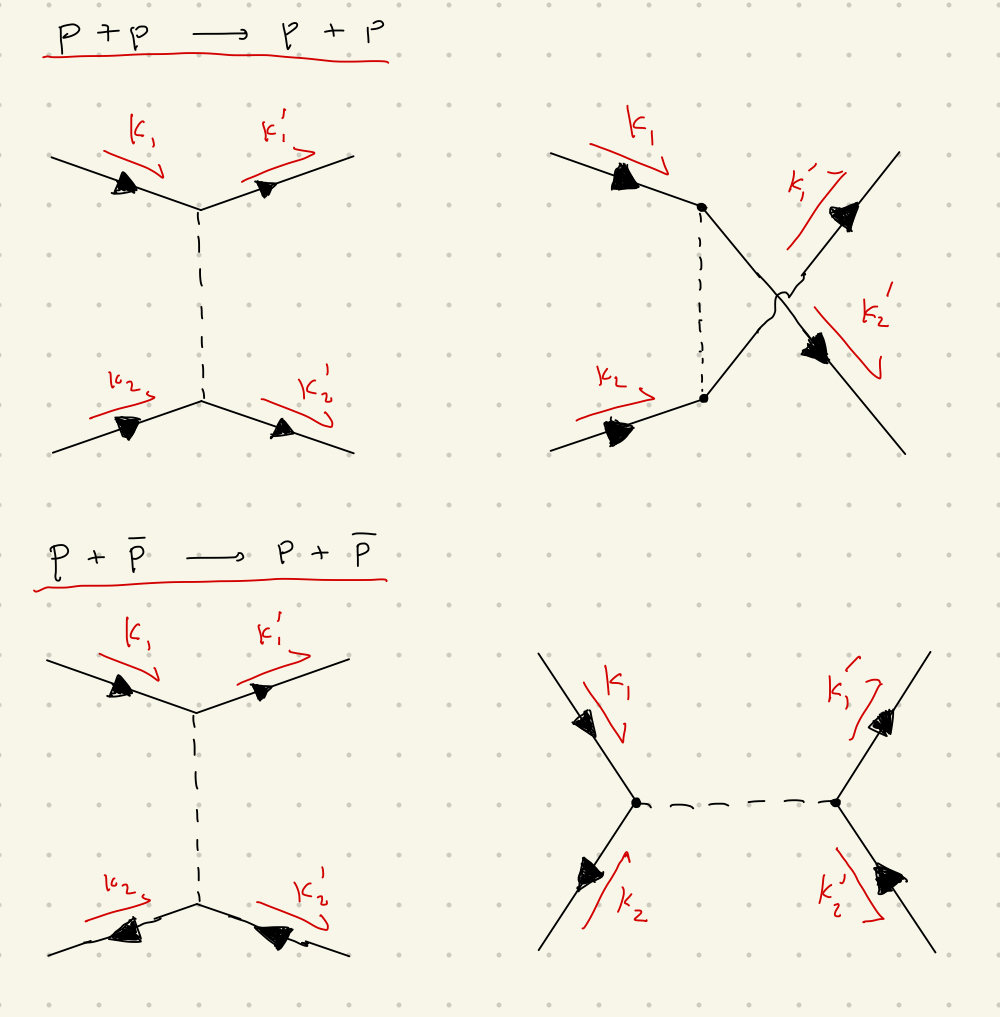
\includegraphics[width=0.5\linewidth]{images/qft-images/yukawastuchannels.jpg}
    \caption{Feynman diagrams for the $\lambda^2$ order 2-2 scattering in $\lambda\psi\overline\psi\phi/3!$ theory. }
    \label{fig:yukawastuchannels}
\end{figure}

\example $2\to 2$ Yukawa scattering. Consider an interaction Lagrangian $\mathcal L=\frac\lambda{3!}\psi^*\psi\phi$. The scattering amplitudes  for $p+p\to p+p$ and $p+\overline p\to p+\overline p$ scattering, as shown in figure \ref{fig:yukawastuchannels} are 
\begin{align*}
    A_{pp\to pp}=-i\lambda^2\left(\frac 1{t-m^2}+\frac 1{u-m^2}\right),\quad A_{p\overline p\to p\overline p}=-i\lambda^2\left(\frac 1{t-m^2}+\frac 1{s-m^2}\right).
\end{align*}

Note that amplitudes should stay the same for $A_{if}=A_{\overline f\overline i}$.

\subsection{Unitarity}
\textcolor{red}{Lec. 16-17}

One consequence of the unitarity of $S$ is the \textbf{optical theorem}. We have 
$$S=\mathbbm 1+iT\implies T-T^\dag=iTT^\dag=iT^\dag T,$$
where $T=(2\pi)^4\delta(k_f-k_i)A_{fi}.$ Inserting the completeness identity and taking the transistional amplitude, we obtain 
$$T_{fi}-T^*_{if}=i\sum_nT_{fn}T^*_{in}=i\sum_nT^*_{nf}T_{ni},$$
where $T^\dag_{fi}=T^*_{if}$. With the delta identity $\delta(k_n-k_f)\delta(k_n-k_i)=\delta(k_i-k_f)\delta(k_i-k_n)$ and $i=f$ (this condition is known as forward scattering), we obtain
\begin{equation}
    \frac 1{2i}(A_{ii}-A^*_{ii})=\Im A_{ii}=\frac 12\sum_n(2\pi)^4\delta(k_i-k_f)\abs{A_{in}}^2=\frac 12\sum_n\int\abs{A_{in}}^2D^{(n)}.
\end{equation}
\example For a 2-2 scattering, $\Im A_{ii}=2k_iE_\text{tot}D_\text{tot}.$

Using the optical theorem, we can examine \textbf{poles} in scattering amplitudes, which correspond to 1-particle intermediate state (hence, $n=1$). Using the optical theorem, 
\begin{align*}
    A_{fi}-A^*_{if}=i\int\frac{\dd^4k}{(2\pi)^3}\delta(k^2-m^2)(2\pi)^4\delta(p_i-k)\bra fA\ket k\bra kA^\dag\ket i=2\pi i\delta(p_i^2-m^2)\bra fA\ket{p_i}\bra{p_i}A^\dag\ket i,
\end{align*}
where we have used $\mathbbm 1=\int\frac{\dd^4k}{(2\pi)^3}\delta(k^2-m^2)\bra k\ket k$ for 1-particle states. Using $\lim_{\epsilon\to 0}\left(\frac 1{x+i\epsilon}-\frac 1{x-i\epsilon}\right)=-2\pi i\delta(x)$, we have 
$$A_{fi}=\Delta(p_i)\bra fA\ket{p_i}\bra{p_i}A^\dag\ket i\implies\Delta(k)=\pm\frac 1{k^2-m^2+i\epsilon}.$$

\example Consider a creation process $m_1+m_2\to m_3$. There is a pole at $s^2-m_3^2$. This is known as \textbf{resonance production}.

Similarly, \textbf{branch cuts} correspond to 2-particle intermediate states. With the optical theorem, 
$$A_{fi}-A^*_{if}=\frac i{64\pi^2}\sqrt{\frac{s-4m^2}s}\theta(s-4m^2)\int\dd\Omega\bra fA\ket{k_1k_2}\bra{k_1k_2}A\ket k.$$
It is clear that there is a square root branch cut starting at $s=4m^2$. To work around branch cuts, it is necessary to use analytic continuation - if $A_{fi}$ and $A^*_{if}$ are equal on $\mathbb R\bigcap [s<4m^2]$, they are equal everywhere except on singularities.:
$$A_{fi}(s)=A^*_{if}(s),\quad s<4m^2\implies A_{fi}(s)=A^*_{if}(s^*),\quad s>4m^2.$$

\example For forward scattering, $A(s)=A^*(s^*)$. For $s=s+i\epsilon$, this states $\Re A(s+i\epsilon)+i\Im A(s+i\epsilon)=\Re A(s-i\epsilon)-i\Im A(s-i\epsilon)$ - the real part is continuous while the imaginary part has a sign discontinuity, $\text{Disc }A=2i\Im A(s+i\epsilon)$. Because of this discontinuity, it is useful to use Feynman prescription, writing $m^2$ ad $m^2-i\epsilon$, which moves the branch cut to slightly under the real axis. 

\textbf{Method of dispersion relations} makes use of poles and branch cuts on $A(s)$ along the real axis to reconstruct the amplitude. For a single branch cut (implying no crossing symmetries), by the Residue theorem, we get 
$$\frac 1{2\pi i}\oint\frac{f(x)}{x-z}\dd z=f(z)=\frac 1{2\pi i}\int^\infty_0\dd x\frac{f(x+i\epsilon)-f(x-i\epsilon)}{x-z}.$$
Since the optical theorem relates Feynman diagrams of order $\lambda^\alpha$ to the imaginary part of $\lambda^{2\alpha}$, we can recursively use dispersion relation to get higher order terms.



\subsection{Renormalization}
\textcolor{red}{Lec. 17-20 but will be using Burdman's notes\footnote{\url{http://fma.if.usp.br/\%7Eburdman/QFT1/lecture_21.pdf}}.}



We define the \textbf{one part irreducible} diagram as a diagram that cannot be disconnected by cutting a single internal line. Then, a full propagator can be written as a geometric series of one part irreducibles:
$$\frac i{p^2-m^2+i\epsilon}+(-i\Pi(p^2))\left(\frac i{p^2-m^2+i\epsilon}\right)^2+(-i\Pi(p^2))^2\left(\frac i{p^2-m^2+i\epsilon}\right)^3+\cdots=\frac i{p^2-m^2-\Pi(p^2)+i\epsilon}.$$

\example Breit-Wigner resonance. First, consider the scattering amplitude $A(p^2)=\bra pA\ket p$ of an unstable particle. It holds that 
$$2i\Im A(p^2)=i\int\abs{\bra{k_1k_2}A\ket p}^2 D^{(2)}\dd(k_1k_2)\implies \Im A(p^2)=m\Gamma.$$ 
Ignoring the real part of $\Pi$, we have $\Im\Pi(p^2=m^2)=-\Im A(p^2=m^2)=-m\Gamma$: the scattering amplitude can be written 
$$A_{fi}\sim \frac 1{2m(E_T-m)+im\Gamma}\implies\sigma\sim\abs{A}^2\sim\frac 1{(E_T-m)^2+\Gamma^2/4}$$

\subsubsection{Mass Renormalization}
We define the \textbf{physical mass} $m$ to be where the pole is in the amplitude, as compared to the mass that appears in the Lagrangian, which we will call the bare mass $m_0$. Therefore, we have 
$$p^2-m_0^2-\left.\Pi(p^2)\right|_{p^2=m^2}=p^2-m_0^2-\left.\left[\lambda^2\Pi^{(2)}(p^2)+\lambda^3\Pi^{(3)}(p^2)+\lambda^4\Pi^{(4)}\cdots\right]\right|_{p^2=m^2}=0,$$
where $-i\Pi^{(n)}$ is the 1 part irreducible scattering amplitude to the $\mathcal O(\lambda^n)$ order.

Evidently, $m^2=m^2(m_0^2,\lambda)$. If we write 
$$m_0^2=m^2+\delta m^2=m^2+\lambda^2(\delta m^{(2)})^2+\lambda^3(\delta m^{(3)})^2+\lambda^4(\delta m^{(4)})^2+\cdots,$$
where $\delta m^2$ is the mass correction, we obtain 
$$\mathcal L=\frac 12\partial_\mu\phi\partial^\mu\phi-\frac{m^2}2\phi^2-\frac{\delta m^2}2\phi^2+\mathcal L_\text{int}.$$
Hence, the effective interaction Lagrangian has a $\delta m^2/2\phi^2$ term, which we will call the \textbf{mass counterterm}. 

\subsubsection{Field Renormalization}
Writing the propagator,
$$\frac i{p^2-m^2-\Pi^\text{full}(p^2)}\sim\frac i{(p^2-m^2)(1-\Pi'(m^2)}\equiv \frac{iZ}{p^2-m^2},\quad z=\frac{1}{1-\Pi'(m^2)}\sim 1+\Pi'(m^2).$$
For the residue to stay constant, we need $\Pi'(m^2)=0$.

From the optical theorem, we see that $\int \dd^4kZ\ket k\bra k=\mathbbm 1$, requiring $\phi\to\frac{\phi_0}{\sqrt Z}$ for the external momenta to be properly normalized. For this, it is convenient to define $Z=1+\delta Z$. 

\subsection{Regularization}
\subsubsection{Momentum Cutoff}
It is possible to evaluate how much an interaction diverges by introducting a cutoff momentum $\Lambda$ to the integrals. The superficial degree of divergence of a $\phi^n$ theory in $d$ dimensions is 
$$D=dL-2I,\quad nV=E+2I,\quad L=I-(V-1)\implies D=d\left(1-\frac 1n\right)E-2\left(1+\frac dn\right)I+d,$$
where there are $E$ external lines, $V$ vertices, $I$ internal lines, and $L$ loops. Given $D$, we say
\begin{itemize}
    \item $D>0$: Super-renormalizable. In EFT, relevant;
    \item $D=0$: Renormalizable. In EFT, marginarlly relevant;
    \item $D<0$: Non-renormalizable. In EFT, irrelevant.
\end{itemize}
In EFT, we let the interaction constant $\lambda$ be dimensionless and match higher order dimensions with cutoff scale $\Lambda$. In EFT, non-renormalizable operators are $p^2/\Lambda^2$ suppressed. 

However, in this perspective, bare mass is given $m^2=\Lambda^2\lambda_2$ where $\lambda_2$ is dimensionless, which means $m_0^2$ is tuned to accuracy $m^2_\text{phys}/\Lambda^2$.

\subsection{Loop Integrals}
\textcolor{red}{Lec. 21}
\subsubsection{Useful Formulae}
Feynman parametrization is given as 
\begin{equation}
    \frac 1{A_1\cdots A_n}=\int^1_0\dd x_1\cdots\dd x_n\cdot\delta\left(\sum x_i-1\right)\frac{(n-1)!}{\left(x_1A_1+\cdots+x_nA_n\right)^n}.
\end{equation}
$d$ dimensional volume element is given as (assuming isotropy)
\begin{equation}
    \dd^dk=\Omega_{d-1}k^{d-1}\dd k=\frac{2\pi^{d/2}}{\Gamma(d/2)}k^{d-1}\dd k.
\end{equation}

\example{$\phi^3$ 1-Loop Diagram.}
The one-loop integral for $\phi^3$ theory is 
\begin{align*}
    iA&=\frac 12(-i\lambda)^2\int_{\mathbb R^{1,3}}\frac{\dd^4k}{(2\pi)^4}\frac{i}{k^2-m^2+i\epsilon}\frac{i}{(k-p)^2-m^2+i\epsilon}\\
    &=\frac{\lambda^2}{2}\int^1_0\dd x\int_{\mathbb R^{1,3}}\frac{\dd^4k}{(2\pi)^4}\frac{1}{[(k^2-m^2)(1-x)+x((k-p)^2-m^2)+i\epsilon]^2}\\
    &=\frac{\lambda^2}{2}\int^1_0\dd x\int_{\mathbb R^{1,3}}\frac{\dd^4k}{(2\pi)^4}\frac{1}{[k^2-(m^2-p^2x(1-x))+i\epsilon]^2}\\
    &=\frac{i\lambda^2}{2}\int^1_0\dd x\int_{\mathbb R^4}\frac{\dd^4k}{(2\pi)^4}\frac{1}{[k^2+a]^2},\quad a=(m^2-p^2x(1-x))\\
    &=\frac{i\lambda^2}{16\pi^2}\int^1_0\dd x\int^\Lambda_0\dd k\frac{k^2}{(k^2+a-i\epsilon)^2}\\
    &=\frac{i\lambda^2}{16\pi^2}\int^1_0\dd x\left(\log\left(\frac{\Lambda^2}{a}\right)-1\right).
\end{align*}


\pagebreak

\section{Spin 1/2 Field Theory}

\subsection{Groups}

The \textbf{Poincare group} $P=\{(\Lambda,a)\}$ with multiplication $(\Lambda_1,a_1)\cdot (\Lambda_2,a_2)=(\Lambda_1\Lambda_2,\Lambda_1a_2+a_1)$ is the group of isometry transformations (Lorentz + translations, $x'=\Lambda x+a$) of the Minkowski spacetime. 

The basic subgroups include homogeneous Lorentz group $L=\{(\Lambda,0)\}$ and translations $T_4=\{(\mathbbm 1,a)\}$.

The \textbf{Lorentz Group} $\{\Lambda\}$ is a matrix group defined $\Lambda^\intercal g\Lambda=g$, where $g$ is the Minkowski $+,-,-,-$ metric. The generators can be written 
$$\Lambda^\intercal g\Lambda=(\mathbbm 1-\omega^\intercal)g(\mathbbm 1-\omega)=g\implies\omega g=-g\omega^\intercal,\quad \omega^{\mu\nu}=-\omega^{\nu\mu}.$$
From antisymmetry, there are 6 real parameters over $\mu\nu$. Per convention, the generators $\omega$ are typically written 
$$-\omega=\frac i2\omega^{\mu\nu}S_{\mu\nu},$$
where $S_{\mu\nu}$ are fixed matrices. Its lie algebra is 
$$\comm{S_{\mu\nu}}{S_{\omega\rho}}=-i(g_{\mu\omega}S_{\nu\rho}+g_{\nu\rho}S_{\mu\omega}-g_{\mu\rho}S_{\nu\omega}-g_{\nu\omega}S_{\mu\rho}).$$

For intuition, the fundamental/vector (1/2,1/2) representation of $S_{\mu\nu}$ is
$$(S_{\mu\nu})^{\lambda\rho}=i(\delta^\lambda_\mu\delta^\rho_\nu-\delta^\lambda_\nu\delta^\rho_\mu).$$
If we define 
\begin{itemize}
    \item $S^{0i}=-S^{i0}=K^i$ generator of boost, $\omega^{i0}=-\omega^{0i}$ rapidity;
    \item $S^{ik}=\epsilon^{ikl}J^l$ generator of rotation, $\omega^{ik}=\epsilon^{ikl}\omega^l$ rotation angle,
\end{itemize}
then 
$$\comm{J^i}{J^k}=i\epsilon^{ikl}J_l,\quad\comm{J^i}{K^i}=i\epsilon^{ikl}K_l,\quad\comm{K^i}{K^l}=i\epsilon^{ikl}J_l.$$
Note that $\{K\}$ isn't a subgroup.

Lastly, because representation preserves structure, we can simply take the matrix exponential to get the finite transformations:
$$\Lambda=\exp\left(\frac i2\omega^{\mu\nu}S_{\mu\nu}\right)=\exp\left(i(\omega\cdot\mathbf J+\omega u\cdot\mathbf K)\right).$$

\subsection{Representations}
First, we introudce fields and states:
\begin{itemize}
    \item \textbf{Fields} are operators on Hilbert space. They are finite dimensional representations of the Lorentz group and transform per the Poincare group. We write
    $$U(\Lambda,a)\circ\phi_\alpha(x)\circ U^{-1}(\Lambda,a)=D_{\alpha\beta}\phi_\beta(\Lambda x+a).$$
    $D_{\alpha\beta}$ is the Lorentz transformation matrix, which isn't necessarily unitary.
    \item \textbf{States} are vectors in Hilbert space. They are representations of the Poincare group and transform per the Lorentz group (states don't necessarily depend on the position.) Therefore, we simply write 
    $$\Lambda:\ket k\to U(\Lambda)\ket k.$$
\end{itemize}

\subsubsection{Representations of the Poincare Group}

We use Wigner's classification on irreducible representations of the Poincare group. Given a state's momentum, we can find orbit $\hat p$ for which there exists $L(p)$ such that $L(p)\ket{\hat p}=\ket p$. The little group denotes the isometry group of $\hat p$ (formally defined $\{\Lambda\}$ such that $\Lambda\hat p=\hat p$.)

\begin{center}
\begin{tabular}{ |c|c|c| } 
\hline
 Orbit/characteristic momentum & $\hat{p}$ & Little group $H\hat{p}$ \\ 
 \hline
 $p^2=m^2,\,p^2>0$ & $(m,0)$ & SO(3) $\sim$ SU(2) \\ 
 \hline
 $p^2=0,\,p^0>0$ & $(1,\hat{e}_3)$ & $E_2$ \\ 
 \hline
 $p=0$ & $(0,0)$ & $L^\uparrow_+\sim\text{SL}(2,\mathbb C)$\\
 \hline
 $p^2=-m^2$ & $(0,m\hat e_3)$ & SU(1,1)\\
 \hline
\end{tabular}
\end{center}

Now, we define the representation of $H\hat p$ as 
$$U(\Lambda)\ket{\hat p,\alpha}=D_{\alpha\alpha'}(\Lambda)\ket{\hat p,\alpha'},\quad\Lambda\in H\hat p.$$

Given the representation of $H\hat p$, we can find the representation of the general $\Lambda\notin H\hat p$ as well. Given $\ket{p,\alpha}\equiv U(L(p))\ket{\hat p,\alpha}$,
\begin{align*}
    U(\Lambda)\ket{p,\alpha}&=\left[U(L(\Lambda p))U(L^{-1}(\Lambda p))\right]U(\Lambda)U(L(p))\ket{\hat p,\alpha}\\
    &=U(L(\Lambda p))\left[U(L^{-1}(\Lambda p))U(\Lambda)U(L(p))\right]\ket{\hat p,\alpha}\\
    &=U(L(\Lambda p))D_{\alpha\alpha'}(L^{-1}(\Lambda p)\Lambda L(p))\ket{\hat p,\alpha}\\
    &=D_{\alpha\alpha'}(L^{-1}(\Lambda p)\Lambda L(p))\ket{\Lambda p,\alpha'}.
\end{align*}
We have used the fact that $U(L^{-1}(\Lambda p))U(\Lambda)U(L(p))$ is a representation of the little group and $D_{\alpha\alpha'}$ is a matrix.

\paragraph{Case 1 - $\hat p=(m,0),\,H\hat p=\text{SO}(3)\sim\text{SU}(2)$}

The SU(2) group can be represented by the particle's $J^2$ and $J_3$ values. We let $\ket{\hat p,\alpha}\to\ket{\hat p,j\sigma}$, where $j$ is total spin and $\sigma$ is the third component. The D matrix is written 
$$U(\Lambda)\ket{p,j\sigma}=D^j_{\sigma\sigma'}(L^{-1}(\Lambda p)\Lambda L(p))\ket{\Lambda p,j\sigma'}.$$

For moving particles, $\comm{J^i}{p^k}=i\epsilon^{ikl}p^l\ne 0$, which necessitates the helicity, defined 
$$\Sigma=\frac{\mathbf J\cdot\mathbf p}{\abs{\mathbf p}}\implies\comm{p^i}{\Sigma}=\comm{p^i}{J^k}\frac{p^k}{\abs{\mathbf p}}=0.$$

Therefore, for moving particles, we write $\ket{p,j\sigma}\to\ket{p,j\lambda}$ with $\Sigma\ket{p,j\lambda}=\lambda\ket{p,j\lambda}.$

\paragraph{Case 2 - $\hat p=(1,\hat e_3),\,H\hat p=E_2$} The $E_2$ group can be written 
$$\Lambda\hat p=\hat p\implies\omega\hat p=0,\quad\begin{pmatrix}0&u^1&u^2&u^3\\-u^1&0&\omega^{12}&\omega^{13}\\-u^2&-\omega^{12}&0&\omega^{23}\\-u^3&-\omega^{13}&-\omega^{23}&0\end{pmatrix}\begin{pmatrix}1\\0\\0\\1\end{pmatrix}=\begin{pmatrix}u_3\\-u_1+\omega^{13}\\-u_2+\omega^{23}\\-u_3\end{pmatrix}.$$
Therefore there are only three generators, $J_3,J_1+K_2,J_2-K_1$. If we let $H^1=J^1+K^2,H^2=J^2-K^1$, the algebra becomes $\comm{J^3}{H^{1,2}}=\pm iH^{2,1}$ and $\comm{H^1}{H^2}=0$, showing $E_2$ is a semidirect product of SO(2) and $T_2$: $E_2=\text{SO}(2)\rtimes T_2$

To find the irreducible representations of $E_2$, we use Wigner's classification again. For $\mathbf H=\begin{pmatrix}H^1\\H^2\end{pmatrix}$ with $\mathbf H\ket{\Pi,\alpha}=\Pi\ket{\Pi,\alpha}$, 
\begin{center}
\begin{tabular}{|c|c|c|}
     \hline
     Orbit & $\hat\Pi$ & $H\hat\Pi$\\
     \hline
     $\Pi^2=c^2$ & $(1,0)$ & $e$; anything\\
     \hline
     $\Pi^2=0$ & $(0,0)$ & SO(2)\\
     \hline
\end{tabular}
\end{center}

$\hat\Pi=(1,0)$ corresponds to continuous spin states, which we will neglect here. 

For $\hat\Pi=(0,0)$, the little group is SO(2), which has a one-dimensional representation $D(R(\omega))=e^{i\omega\lambda}$ with $\lambda=0,\pm\frac 12,\pm 1,\pm\frac 32,\cdots$.

Therefore, for massless particles, we write $\ket{p,\alpha}\to\ket{p,\lambda}$ with 
$$U(\Lambda)\ket{p,\lambda}=e^{i\lambda\omega}(L^{-1}(\Lambda p)\Lambda L(p))\ket{\Lambda p,\lambda}.$$

$\lambda$ is called the helicity. Note that $\gamma$ doesn't have spin.

\paragraph{Case 3 - $\hat p=(0,0)$, $H\hat p=L^\uparrow_+$}

This case corresponds to the vacuum states. For simplicity, we choose the trivial representation $\ket 0$.

\subsubsection{Weyl Spinor Representation of $\mathrm{SL}(n,\mathbbm C)\sim L^\uparrow_+$}

Consider the Pauli matrices,
$$\sigma^1=\begin{pmatrix}&1\\1&\end{pmatrix},\quad\sigma^2=\begin{pmatrix}&-i\\i&\end{pmatrix},\quad\sigma^3=\begin{pmatrix}1&\\&-1\end{pmatrix}.$$
We define the 4-pauli vectors as 
$$\sigma^\mu=(\mathbbm 1,\boldsymbol\sigma)\implies\sigma_\mu=(\mathbbm 1,-\boldsymbol\sigma),\quad\overline\sigma^\mu=(\mathbbm 1,-\boldsymbol\sigma).$$
If we consider the 2x2 matrices $[x]=x^\mu\sigma_\mu$, for $A\in\mathrm{SL}(2,\mathbb C)$, we have that $[x]_A=A[x]A^\dag$ is a Lorentz transformation; 
$$\det[x]=x^2,\quad x^2_A=\det[x]_A=\det(A[x]A^\dag)=x^2.$$
From this, we can find four different representations for $L^\uparrow_+$:
\begin{itemize}
    \item Trivial representation; $\psi_\alpha\to A\indices{_\alpha^\beta}\psi_\beta\sim A\psi$
    \item Conjugate representation; $\psi_{\dot\alpha}\to(A^*)\indices{_{\dot\alpha}^{\dot\beta}}\psi_{\dot\beta}\sim \psi A^\dag$
    \item Transpose representation $\psi^\alpha\to ({A^\intercal}^{-1})\indices{^\alpha_\beta}\psi^\beta\sim\psi A^{-1}$
    \item Hermite representation $\psi^{\dot\alpha}\to\bar A\indices{^{\dot\alpha}_{\dot\beta}}\psi^{\dot\beta}\sim\bar A\psi$. We define $\bar A=(A^\dag)^{-1}$.
\end{itemize}
Note that, because $L^\uparrow_+$ has $\det=1$, $A^{-1}=A^\intercal$ and therefore we only have lower indices. If we had a unitary representation, $\bar A=A$, and would've only undotted indices.

Further, note that we use the levi-civita symbol to lower and raise indices:
$$\epsilon^{\alpha\beta}=\epsilon_{\alpha\beta}=\epsilon^{\dot\alpha\dot\beta}=\epsilon_{\dot\alpha\dot\beta}=\begin{pmatrix}&1\\-1&\end{pmatrix}.$$

From the condition that $\det A=1$, the generators must be such that $\Tr \omega=0\implies\omega=\frac i2(\boldsymbol\alpha+i\boldsymbol\beta)\cdot\boldsymbol\sigma$. Then, 
$$A=\exp\left(\frac i2(\boldsymbol\alpha+i\boldsymbol\beta)\cdot\boldsymbol\sigma)\right),\quad\bar A=\exp\left(\frac i2\left(\boldsymbol\alpha-i\boldsymbol\beta\right)\cdot\boldsymbol\sigma\right).$$
Therefore, the general representation of $\mathrm{SL}(2,\mathbb C)\sim L^\uparrow_+$ is 
$$D^{m,n}=\varphi\indices{_{\alpha_1\cdots\alpha_m}^{\dot\beta_1\cdots\dot\beta_n}}=\exp\left(\frac i2(\boldsymbol\alpha+i\boldsymbol\beta)\cdot\boldsymbol\sigma\right)\exp\left(\frac i2\left(\boldsymbol\alpha-i\boldsymbol\beta\right)\cdot\boldsymbol\sigma\right).$$

Another way to derive is to start by rewriting $\mathbf M=\frac 12(\mathbf J+i\mathbf K),\quad\mathbf N=\frac 12(\mathbf J-i\mathbf K)$. By writing this, $\mathbf M$ and $\mathbf N$ commute with each other and have their own $\mathfrak{su}(2)$ algebra. Therefore, 
$$\Lambda=e^{i(\mathbf\omega\cdot\mathbf J+\mathbf v\cdot\mathbf k)}=e^{i\mathbf M\cdot(\mathbf w-i\mathbf v)}e^{i\mathbf N\cdot(\mathbf w+i\mathbf v)}.$$

We now consider the (1/2,0) representation. We have 
$$\mathbf M=\frac{\sigma}2,\quad\mathbf N=0\implies\mathbf J=\frac{\sigma}2,\quad\mathbf K=-\frac{i\sigma}2.$$
The objects transform under this representation are called left-handed spinors $\psi_L$. These transform
$$(\psi_L)_\alpha\to A\indices{_\alpha^\beta}\psi_\beta,\quad A\indices{_\alpha^\beta}=\exp\left(i\frac{w\cdot\sigma}{2}+\frac{u\cdot\sigma}2\right).$$

Similarly, the (0,1/2) representation has
$$M=\frac{\sigma}2,\quad N=0\implies J=\frac{\sigma}2,\quad K=\frac{i\sigma}2.$$
The objects that transform under this representation are called right-handed spinors $\psi_R$. These transform
$$(\psi_R)^{\dot\beta}\to\bar A\indices{^{\dot\alpha}_{\dot\beta}}(\psi_R)^{\dot\beta},\quad\bar A\indices{^{\dot\alpha}_{\dot\beta}}=\exp\left(i\frac{w\cdot\sigma}2-\frac{u\cdot\sigma}2\right).$$

Lastly, the (1/2,1/2) representation can be written 
$$(\psi_L)^\alpha(\sigma^\mu)_{\alpha\dot\beta}(\psi_R)^{\dot\beta}.$$
This is an ordinary 4-vector; recall that $x^\mu\sim [x]\to A[x]A^\dag$.

\subsubsection{Dirac Spinor Representation}

For theories with parity symmetry, Dirac spinors are used to include both Left-handed spinors as well as Right-handed spinors. We let $\psi=\begin{pmatrix}\chi_\alpha\\\bar\psi^{\dot\alpha}\end{pmatrix}$. The Lorentz transformation is 
\begin{align*}
    D(\Lambda)&=\begin{pmatrix}\exp\left(\frac i2\boldsymbol\sigma(\boldsymbol\omega-i\mathbf u)\right)&0\\0&\exp\left(\frac i2\boldsymbol\sigma(\boldsymbol\omega+i\mathbf u)\right)\end{pmatrix}\\
    &=\exp\left(i\boldsymbol\omega\cdot\boldsymbol\Sigma+\frac 12\mathbf u\cdot\boldsymbol\alpha\right),\quad\boldsymbol\Sigma=\frac 12\begin{pmatrix}\boldsymbol\sigma&0\\0&\boldsymbol\sigma\end{pmatrix},\quad\boldsymbol\alpha=\begin{pmatrix}-\boldsymbol\sigma&0\\0&\boldsymbol\sigma\end{pmatrix}.
\end{align*}
$\boldsymbol\Sigma$ is a representation of $\mathbf J$, and $\boldsymbol\alpha$ is a representation of $\mathbf K$. The generator algebra is such that
$$\Sigma^i\Sigma^k=\alpha^i\alpha^k=\delta^{ik}+i\epsilon^{ikl}\Sigma^l,\quad\comm{\Sigma^i}{\gamma^0}=\comm{\alpha^i}{\gamma^0}=0.$$

where
$$\gamma^0=\begin{pmatrix}0&\mathbbm 1\\\mathbbm 1&0\end{pmatrix},\quad\gamma^i=\begin{pmatrix}0&\sigma^i\\-\sigma^i&0\end{pmatrix}.$$
These are known as the Dirac gamma matrices. These have an algebra,
$$\acomm{\gamma^\mu}{\gamma^\nu}=2g^{\mu\nu}\times\mathbbm 1.$$

\subsection{Formalism}
We want a Lagrangian that:
\begin{itemize}
    \item Is Lorentz invariant,
    \item Has at most 2 derivatives and 2 fields,
    \item Has a real action,
    \item Has a U(1) symmetry ($\chi\to e^{i\alpha}\chi$). Experimentally, every 1/2 has a conserved charge, for example, leptop/baryon number, electric charge.
\end{itemize}

The kind of left-handed objects we can have are 
$$\chi_\alpha,\quad\chi^*_{\dot\alpha},\quad\partial^\mu,\quad\sigma^\mu_{\alpha\dot\alpha},\quad\bar\sigma^{\mu\dot\alpha\alpha},\quad\epsilon_{\alpha\beta}.$$

For a bilinear $\mathcal L$, there are three possibilities:
\begin{enumerate}
    \item $\mathcal L=c\chi^*_{\dot\alpha}\bar\sigma^{\mu\dot\alpha\dot\beta}(\partial_\mu\chi_\beta)$. Taking the complex conjugate then integrating by parts, realness requires that $c^*$ is purely imaginary; from convention, we choose $c=i$.
    \item $\mathcal L=\chi_\alpha\epsilon^{\alpha\beta}\chi_\beta$. This is not U(1) invariant. This corresponds to the Majonara mass, for neutrinos without charge.
    \item $(\partial_\mu\chi_\alpha)\epsilon^{\alpha\beta}(\partial^\mu\chi_\beta)$. This is not U(1) invariant either.
\end{enumerate}
Therefore, we write the action
\begin{equation}
    S=\int\dd^4x\,i\chi^*_{\dot\alpha}\bar\sigma^{\mu\dot\alpha\alpha}(\partial_\mu\chi_\alpha)=\int\dd^4x\,i\bar\chi\slashed\partial\chi,\quad\slashed\partial\equiv\bar\sigma^\mu\partial_\mu.
\end{equation}

From the Euler-Lagrange equation, we obtain
\begin{equation}
    \bar\sigma^{\mu\dot\alpha\beta}\partial_\mu\chi_\beta=0,
\end{equation}
known as the (left-handed) Weyl equation.

This is consistent with the massless Klein-Gordon equation. 

The plain wave solution is 
\begin{align*}
    \chi_L&=\int\frac{\dd^3p}{\sqrt{(2\pi)^32\omega_p}}\left[a_{p_-}\begin{pmatrix}0\\1\end{pmatrix}e^{-ipx}+b^\dag_{p_+}\begin{pmatrix}1\\0\end{pmatrix}e^{ipx}\right]\\
    \chi_L^\dag&=\int\frac{\dd^3p}{\sqrt{(2\pi)^32\omega_p}}\left[a^\dag_{p_-}\begin{pmatrix}0\\1\end{pmatrix}e^{ipx}+b_{p_+}\begin{pmatrix}1\\0\end{pmatrix}e^{-ipx}\right].
\end{align*}

Similarly, the right-handed Lagrangian and the corresponding equation are
$$\mathcal L=\pm i\psi^{*\alpha}\sigma^\mu_{\alpha\dot\beta}(\partial_\mu\psi^{\dot\beta})\implies\sigma^\mu_{\alpha\dot\beta}\partial_\mu\psi^{\dot\beta}=0.$$
The plain wave solution is
$$\psi_R=\int\frac{\dd^3p}{\sqrt{(2\pi)^32\omega_p}}\left[a_{p-}\begin{pmatrix}1\\0\end{pmatrix}e^{-ipx}+b^\dag_{p_+}\begin{pmatrix}0\\1\end{pmatrix}e^{ipx}\right].$$


\subsubsection{Majorana Theory}
To add mass to our theory, we consider the Majorana mass term. The corresponding action is 
$$S=\int\dd^4x\left[i\psi^*_{\dot\alpha}\bar\sigma^{\mu\dot\alpha\alpha}\partial_\mu\psi_\alpha-\frac m2\psi_\alpha\epsilon^{\alpha\beta}\psi_\beta+\text{h.c.}\right].$$
The equations of motion are
$$i\bar\sigma^{\mu\dot\alpha\beta}\partial_\mu\psi_\beta=m(\psi^*)^{\dot\alpha},\quad -i\partial_\mu\psi^*_{\dot\alpha}\bar\sigma^{\mu\alpha\beta}=m\psi^\beta.$$
With the ansatz $\psi_\beta=x_\beta e^{-ipx}+y_\beta e^{ipx}$, we can reduce the equations to 
$$(p\cdot\bar\sigma)x=my^\dag,\quad (p\cdot\bar\sigma)y=-mx^\dag,\iff(p\cdot\sigma)y^\dag=mx,\quad(p\cdot\sigma)x^\dag=-my.$$
The solutions are such that 
$$x_\alpha(p,s)=\sqrt{p\cdot\sigma}\chi_s,\quad y_\alpha(p,s)=(2s)\sqrt{p\cdot\sigma}\chi_s,$$
giving us 
$$\psi_\alpha(x)=\int\frac{\dd^3p}{\sqrt{(2\pi)^32\omega_p}}\sum_s\left(x_\alpha(p,s)a_{p,s}e^{-ipx}+y_\alpha(p,s)a^\dag_{p,s}e^{ipx}\right).$$

\subsection{Dirac Theory}

\subsubsection{Gamma Matrices}

We define the Dirac gamma matrices (in \textbf{Weyl/Chiral basis}):

$$\gamma=\begin{pmatrix}0&\sigma^\mu\\\overline\sigma^\mu&0\end{pmatrix}$$

The gamma matrices have a Clifford algebra:
$$\acomm{\gamma^\mu}{\gamma^\nu}=2g^{\mu\nu}\mathbbm 1.$$

\subsubsection{Dirac Formalism}

To add mass to the theory while keeping U(1) symmetry, we consider a Lagrangian of the form 
$$\mathcal L=i(\psi^\dag_L)_{\dot\alpha}\overline\sigma^{\mu\alpha\dot\beta}\psi_{L\beta}+(\psi^\dag_R)^\alpha\sigma^\mu_{\dot\alpha\beta}\partial_\mu\psi^{\dot\beta}_R-m(\psi^\dag_R)^\alpha(\psi_{L\beta})+\text{h.c.}.$$

\pagebreak

\section{Path Integral Formulation}

\subsection{Derivation}

We claim that the propagation amplitude can be written as a functional integral of the exponent of the action:
\begin{equation}
    U(x_a,x_b;T)=\int\mathcal Dx(t)e^{iS[x(t)]/\hbar}.
    \label{41a}
\end{equation}
In the classical limit ($S[x]\gg\hbar$), this makes sense because $\frac{\delta S[x(t)]}{\delta x(t)}=0$ by the method of stationary phase, agreeing with the principle of least action. 

In a more practical form, \eqref{41a} can be written as 
\begin{align}
    \begin{split}
        U(q_0,q_N;T)&=\left(\prod_{i,k}\int\frac{\dd q^i_k\dd q^i_k}{2\pi}\right)\exp\left[i\sum_{i,k}p^i_k(q^i_{k+1}-q^i_k)-\epsilon H\left(\frac{q_{k+1}+q_k}{2},p_k\right)\right]\\
        &=\left(\prod_i\int\mathcal Dq(t)\mathcal Dp(t)\right)\exp\left[i\int^T_0\dd t\left(\sum_ip^i\dot q^i-H(q,p)\right)\right].
    \end{split}
\end{align}

\subsection{Quantization of Scalar Fields}
The correlation function, in terms of path integrals, is 
\begin{equation}
    \bra\Omega T\phi_H(x_1)\phi_H(x_2)\ket\Omega=\lim_{T\to\infty(1-i\epsilon)}\frac{\int\mathcal D\phi\phi(x_1)\phi(x_2)\exp\left[i\int^T_{-T}\dd^4x\mathcal L\right]}{\int\mathcal D\phi\exp\left[i\int^T_{-T}\dd^4x\mathcal L\right]}\label{4correlation}
\end{equation}
Consider a non-interacting real scalar field ($\mathcal L_0=\frac 12(\partial_\mu\phi)^2-\frac 12m^2\phi^2.$) In the momentum space, defined 
$$\phi(x_i)=\frac 1V\sum_{n}e^{-ik_n\cdot x_i}\phi(k_n),$$
where the $n>0$ comes from $\phi^*(k)=\phi(-k)$. The denominator can be written 
\begin{align*}
    \int\mathcal D\phi e^{iS_0}&=\left(\prod_{k^0>0}\int\dd(\Re\phi_n)\dd(\Im\phi_n)\right)\exp\left[-\frac iV\sum_{k^0>0}(m^2-k^2_n)\abs{\phi_n}^2\right]=\prod_{\text{all }k_n}\sqrt{\frac{i\pi V}{k^2_n-m^2+i\epsilon}}.
\end{align*}
We can write our result using the \textbf{functional determinant}. Consider the integral
\begin{equation}
    \left(\prod_k\int\dd\xi_k\right)\exp\left[-\xi_iB_{ij}\xi_j\right]\propto\left[\det B\right]^{-1/2},
\end{equation}
which allows us to write 
\begin{equation}
    \int\mathcal D\phi e^{iS_0}\propto\left[\det(m^2+\partial^2)\right]^{-1/2}.
\end{equation}
Similarly, the numerator can be written 
\begin{align*}
    \int\mathcal D\phi\phi(x_1)\phi(x_2)e^{iS_0}=&\frac 1{V^2}\sum_{m,l}e^{-i(k_m\cdot x_1+k_l\cdot x_2)}\left(\prod_{k^0_n>0}\int\dd(\Re\phi_n)\dd(\Im\phi_n)\right)\cdot(\Re\phi_m+i\Im\phi_m)(\Re\phi_l+i\Im\phi_l)\\
    &\qquad\cdot\exp\left[-\frac iV\sum_{k^0_n>0}(m^2-k^2_n)\left[(\Re\phi_n)^2+(\Im\phi_n)^2\right]\right]\\
    =&\frac 1{V^2}\sum_me^{-ik_m\cdot(x_1-x_2)}\left(\prod_{k^0_n>0}\frac{-i\pi V}{m^2-k_n^2}\right)\frac{-iV}{m^2-k_m^2-i\epsilon},
\end{align*}
where we have used the fact that unless $k_m=-k_l$, the integrand is odd ($k_m=k_l$ cancels $\Re^2$ with $\Im^2$.) 

Taking the continuum limit of the fraction, we obtain
\begin{equation}
    \bra 0T\phi(x_1)\phi(x_2)\ket 0=\int\frac{\dd^4k}{(2\pi)^4}\frac{ie^{-ik\cdot(x_1-x_2)}}{k^2-m^2+i\epsilon}.
\end{equation}
Similarly, the four-point function is nonzero for when two of its fields are equal but opposite in sign.

It is useful to consider the \textbf{generating functional} when computing the correlation functions. We define 
\begin{equation}
    Z[J]\equiv\int\mathcal D\phi\exp\left[i\int\dd^4x\left[\mathcal L+J(x)\phi(x)\right]\right].
\end{equation}
The two-point function is simply 
\begin{equation}
    \bra 0T\phi(x_1)\phi(x_2)\ket 0=\left.\frac 1{Z[J=0]}\left(\frac 1{i^2}\frac{\delta^2}{\delta J(x_1)\delta J(x_2)}\right)Z[J]\right|_{J=0},
\end{equation}
from \eqref{4correlation}.

For the free scalar field theory, we can explicitly find the generating functional. 
\begin{align*}
    Z[J]&\equiv\int D\phi\exp\left[i\int\dd^4x\left[\frac 12\phi(-\partial^2-m^2+i\epsilon)\phi+J(x)\phi(x)\right]\right]\\
    &=\int\mathcal D\phi'\exp\left[i\int\dd^4x\left[\frac 12\phi'(-\partial^2-m^2+i\epsilon)\phi'-\frac 12J(-\partial^2-m^2+i\epsilon)^{-1}J\right]\right]\\
    &=Z_0\exp\left[-\frac 12\int\dd^4x\int\dd^4yJ(y)D_F(y-x)J(x)\right]
\end{align*}
where $\phi'=\phi+(-\partial^2-m^2+i\epsilon)^{-1}J$. Note that to compute $(-\partial^2-m^2+i\epsilon)^{-1}$ we need to work in the momentum space.

The four-point function is then 
\begin{align*}
    \bra 0T\phi(x_1)\phi(x_2)\phi(x_3)\phi(x_4)\ket 0&=\frac 1{Z_0}\prod^4_{j=1}\left(\frac 1i\frac{\delta}{\delta J(x_j)}\right)e^{-\frac 12J_xD_{xy}J_y}\\
    &=\frac 1{Z_0}\prod^3_{j=1}\left(\frac 1i\frac{\delta}{\delta J(x_j)}\right)\left(-J_xD_{x4}e^{-\frac 12J_xD_{xy}J_y}\right)\\
    &=\frac 1{Z_0}\prod^2_{i=1}\left(\frac 1i\frac{\delta}{\delta J(x_j)}\right)\left(\left(-D_{34}+J_xD_{x4}J_yD_{y3}\right)e^{-\frac 12J_xD_{xy}J_y}\right)\\
    &=\frac 1{Z_0}\prod^1_{j=1}\left(\frac 1i\frac\delta{\delta J(x_j)}\right)\left(\left(J_xD_{x2}D_{34}+D_{24}J_yD_{y3}+J_xD_{x4}D_{23}\right)e^{-\frac 12J_xD_{xy}J_y}\right)\\
    &=(D_{12}D_{34}+D_{24}D_{13}+D_{14}D_{23}).
\end{align*}    

\subsection{Quantization of EM Field}
The functional integral  for the electromagnetic theory is 
$$\int\mathcal DAe^{iS[A]},\quad S=\int\dd^4x\left[-\frac 14(F_{\mu\nu})^2\right]=\frac 12\int\dd^4xA_\mu(\partial^2g^{\mu\nu}-\partial^\mu\partial^\nu)A_\nu.$$
This expression vanishes if $\tilde A_\mu=k_\mu\alpha(k)$ for any scalar function $\alpha(k)$, meaning the path integral is badly divergent.

Let $G(A)=0$ be a gauge-fixing condition; for example, $G(A)=\partial_\mu A^\mu$ for Lorentz gauge. We consider the identity 
\begin{equation}
    1=\int\mathcal D\alpha(x)\delta(G(A^\alpha))\det\left(\frac{\delta G(A^\alpha)}{\delta\alpha}\right),\quad A^\alpha_\mu(x)=A_\mu(x)+\frac 1e\partial_\mu\alpha(x).
\end{equation}
Note that $\det\left(\frac{\delta G(A^\alpha)}{\delta\alpha}\right)=\det\left(\frac{\partial^2}e\right)$ is constant. With this condition, the functional integral becomes 
\begin{equation}
    \int\mathcal DAe^{iS[A]}=\det\left(\frac{\delta G(A^\alpha)}{\delta\alpha}\right)\int\mathcal D\alpha\int\mathcal DAe^{iS[A]}\delta(G(A)),
\end{equation}
where we have used the gauge invariance of $S$ and the fact that $A\to A^\alpha$ is a simple shift. Consider letting $G(A)=\partial^\mu A_\mu(x)-\omega(x)$ for a generalization of the Lorentz gauge condition and integrate over all $\omega(x)$ with a weighting function:
\begin{align*}
    \int\mathcal DAe^{iS[A]}&=N(\xi)\int\mathcal D\omega\exp\left[-i\int\dd^4x\frac{\omega^2}{2\xi}\right]\det\left(\frac 1e\partial^2\right)\left(\mathcal D\alpha\right)\int\mathcal DAe^{iS[A]}\delta(\partial^\mu A_\mu-\omega(x))\\
    &=N(\xi)\det\left(\frac 1e\partial^2\right)\left(\int\mathcal D\alpha\right)\int\mathcal DAe^{iS[A]}\exp\left[-i\int\dd^4x\frac 1{2\xi}(\partial^\mu A_\mu)^2\right].
\end{align*}
Hence, the correlation function is 
\begin{equation}
    \bra\Omega T\mathcal O(A)\ket\Omega=\lim_{T\to\inf(1-i\epsilon)}\frac{\int\mathcal DA\mathcal O(A)\exp\left[i\int^T_{-T}\dd^4x\left[\mathcal L-\frac 1{2\xi}(\partial^\mu A_\mu)^2\right]\right]}{\int\mathcal DA\exp\left[i\int^T_{-T}\dd^4x\left[\mathcal L-\frac 1{2\xi}(\partial^\mu A_\mu)^2\right]\right]}.
\end{equation}
The photon propagator is 
\begin{equation}
    \tilde D^{\mu\nu}_F(k)=-\frac{-i}{k^2+i\epsilon}\left(g^{\mu\nu}-(1-\xi)\frac{k^\mu k^\nu}{k^2}\right).
\end{equation}

\end{document}